% Build: lualatex -interaction=nonstopmode -halt-on-error main.tex
\documentclass[12pt,a4paper]{article}

\usepackage{fontspec,polyglossia}
\setdefaultlanguage{ukrainian}
\setmainfont{NewCM10-Regular.otf}[
  BoldFont=NewCM10-Bold.otf,
  ItalicFont=NewCM10-Italic.otf,
  BoldItalicFont=NewCM10-BoldItalic.otf
]
\setsansfont{Noto Sans}
\setmonofont{Noto Sans Mono}[Scale=0.82]

\usepackage{xurl}
\usepackage{geometry,graphicx,booktabs,array,enumitem,caption,titlesec,xcolor,fvextra,float}
\geometry{left=2cm,right=2cm,top=2cm,bottom=2cm}
\setlength{\parindent}{1.25cm}
\setlength{\parskip}{4pt}
\setlength{\emergencystretch}{3em}
\linespread{1.08}
\titleformat{\section}{\normalfont\fontsize{14}{16}\selectfont\bfseries}{\thesection}{0.6em}{}
\titleformat{\subsection}{\normalfont\fontsize{12}{14}\selectfont\bfseries}{\thesubsection}{0.6em}{}
\captionsetup{hypcap=false,font=small,labelfont=bf,labelsep=endash}
\DefineVerbatimEnvironment{code}{Verbatim}{fontsize=\footnotesize,breaklines=true,breakanywhere=true,frame=single,framesep=2mm}

\usepackage[
  unicode,
  colorlinks=true,
  linkcolor=black,
  urlcolor=blue,
  pdfauthor={Давидчук Артем},
  pdftitle={Архітектура комп'ютерів. Частина 2. Лабораторна робота №6}
]{hyperref}

\begin{document}

\pagenumbering{gobble}
\begin{titlepage}
  \begin{center}
    
\includegraphics[width=0.7\textwidth]{../../../../../../templates/letterhead.png}\\[1em]
    \large
    Національний технічний університет України\\
    «Київський політехнічний інститут імені Ігоря Сікорського»\\[1em]
    Факультет інформатики та обчислювальної техніки\\
    Кафедра обчислювальної техніки
  \end{center}

  \vfill
  \begin{center}
    \textbf{\LARGE Архітектура комп'ютерів}\\[0.4em]
    \textbf{\Large Частина 2. Процесори}\\[2em]
    \textbf{\Large Лабораторна робота №6}\\[0.7em]
    \parbox{0.9\textwidth}{\centering
      «Дебаггінг завантажуваного модуля ядра Linux»}
  \end{center}

  \vfill
  \begin{flushright}
    Виконав: студент групи ІО-41\\
    \textit{Давидчук Артем}\\[1em]
    Перевірив: \textit{Каплунов А.~В.}
  \end{flushright}

  \vfill
  \begin{center}Київ --- 2026\end{center}
\end{titlepage}
\pagenumbering{arabic}

\section{Мета роботи}

Ознайомитися з діагностикою помилок у завантажуваних модулях ядра Linux,
структурою повідомлення Oops, адресами секцій модуля у sysfs та зіставленням
адрес машинних інструкцій із рядками вихідного коду. Практично перевірити
\texttt{BUG\_ON()}, обробку помилки виділення пам'яті, \texttt{addr2line} і
\texttt{objdump} у середовищі QEMU для ARMv7.

\section{Постановка задачі}

Із двох запропонованих варіантів обрано завдання 1. Реалізацію модуля з
лабораторної роботи №4 потрібно змінити таким чином:

\begin{enumerate}[leftmargin=*]
  \item для неприпустимого значення параметра використати
    \texttt{BUG\_ON()} замість повідомлення та повернення
    \texttt{-EINVAL};
  \item штучно відтворити ситуацію, коли п'ятий виклик
    \texttt{kmalloc()} повертає \texttt{NULL};
  \item додати до системи збирання налагоджувальну інформацію,
    дизасемблювання та визначення рядка коду за адресою;
  \item отримати обидва діагностичні повідомлення, дослідити стан модуля,
    адреси його секцій і знайти місце аварії.
\end{enumerate}

Репозиторій із вихідним кодом і Makefile:
\begin{center}
\href{https://github.com/davidchyk/university_roadmap/tree/main/semester5/ca2/work/labs/lab6}{github.com/davidchyk/university\_roadmap/.../ca2/work/labs/lab6}
\end{center}

\section{Теоретичні відомості}

\subsection{BUG\_ON та повідомлення Oops}

Макрос \texttt{BUG\_ON(condition)} перевіряє умову і, коли вона істинна,
виконує спеціальну аварійну інструкцію. Ядро формує Oops із номером процесу,
станом регістрів, лічильником команд PC, стеком викликів, кодом інструкцій і
переліком завантажених модулів. У цій роботі умова спрацьовує під час
\texttt{module\_init()}, тому ініціалізація не завершується, а модуль
залишається у проміжному стані \texttt{Loading}.

Oops пошкоджує лише контекст процесу \texttt{insmod}; тестова система
продовжує роботу, що дає змогу прочитати журнал, sysfs і виконати додаткові
команди. Проте такий модуль неможливо штатно вивантажити.

\subsection{Секції модуля та адреса аварії}

Ядро розміщує секції модуля за динамічними адресами. Їх можна прочитати у
\path{/sys/module/hello/sections/}; імена прихованих файлів починаються з
крапки, наприклад \texttt{.init.text}. Для аварії отримано:

\begin{code}
PC = 0xbf005018
.init.text = 0xbf005000
offset = PC - base = 0x18
\end{code}

Файл \texttt{hello.ko} є переміщуваним ELF, тому для визначення рядка
потрібно передати не абсолютну адресу, а зміщення всередині відповідної
секції:

\begin{code}
arm-eabi-addr2line -e hello.ko -j .init.text -f -i 0x18
\end{code}

\subsection{Штучна помилка виділення пам'яті}

Звичайна помилка \texttt{kmalloc()} обробляється без аварії ядра: модуль
звільняє вже створені елементи списку та повертає \texttt{-ENOMEM}.
\texttt{insmod} перетворює цей код на повідомлення
\texttt{Cannot allocate memory}. Така перевірка показує різницю між
контрольованим поверненням помилки й навмисним порушенням інваріанта через
\texttt{BUG\_ON()}.

\section{Програмна реалізація}

\subsection{Аварія для неприпустимого параметра}

Перевірку з ЛР №4 замінено одним викликом:

\begin{code}
BUG_ON(count > 10);
\end{code}

Для тестування передано \texttt{count=11}. У конфігурації ядра ввімкнено
\path{CONFIG_DEBUG_BUGVERBOSE}, тому Oops одразу містить повний шлях і
номер рядка аварії.

\subsection{Імітація відмови kmalloc}

Під час формування п'ятого елемента замість виклику алокатора примусово
присвоюється \texttt{NULL}. Для попередніх елементів викликається справжній
\texttt{kmalloc()}.

\begin{code}
event = i == 4 ? NULL : kmalloc(sizeof(*event), GFP_KERNEL);
if (!event) {
    pr_err("memory allocation failed for message %u\n", i + 1);
    free_events(false);
    return -ENOMEM;
}
\end{code}

Таким чином, для \texttt{count=5} у журналі мають з'явитися чотири
привітання, після чого ініціалізація завершиться контрольованою помилкою.

\subsection{Зміни системи збирання}

До Kbuild додано ключ \texttt{-g}, який зберігає DWARF-відомості у
\texttt{hello.ko}:

\begin{code}
ccflags-y += -g
obj-m := hello.o
\end{code}

Makefile містить цілі \texttt{disasm} і \texttt{locate}. Перша формує
поєднане дизасемблювання з вихідним кодом, друга запускає
\texttt{addr2line} для секції \texttt{.init.text}:

\begin{code}
disasm: all
    $(CROSS_TOOLS)objdump -drS hello.ko > hello.disasm

locate: all
    $(CROSS_TOOLS)addr2line -e hello.ko \
        -j .init.text -f -i $(ADDR)
\end{code}

\section{Збирання та запуск}

Модуль перевірено \texttt{checkpatch.pl}: отримано
\texttt{0 errors, 0 warnings}. Він зібраний GNU Arm Toolchain 8.3 для
Linux 4.19.325/ARMv7. Команда \texttt{file} підтвердила наявність
\texttt{debug\_info}, а \texttt{vermagic} збігається з ядром QEMU.

\begin{figure}[H]
  \centering
  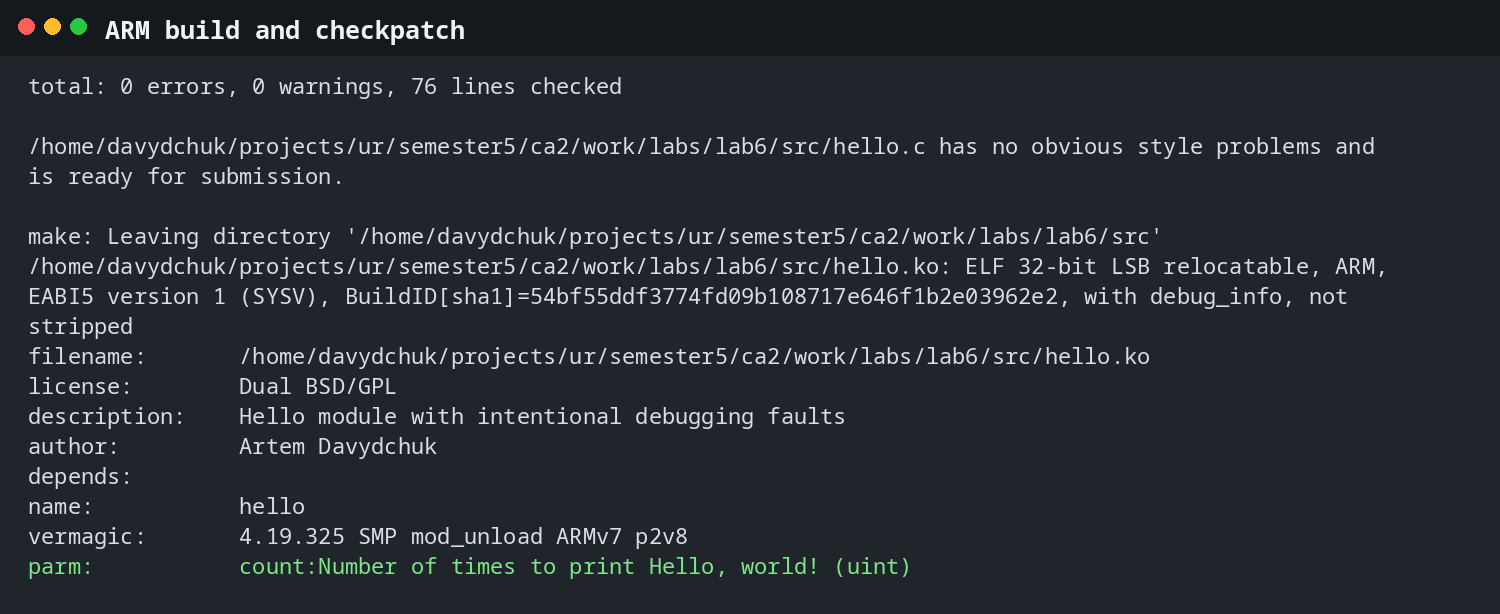
\includegraphics[width=\textwidth]{media/build-and-modinfo.png}
  \caption{Перевірка стилю, тип модуля та modinfo}
\end{figure}

Для кожного дефекту використано окрему сесію QEMU, щоб стан модуля після
\texttt{BUG\_ON()} не впливав на інший тест. Запуск виконувався для машини
\texttt{virt} з 512 МБ пам'яті, ядром із ЛР №3 і окремою копією initramfs,
до якої додано \texttt{hello.ko}.

\section{Результати дебаггінгу}

\subsection{Контрольована відмова виділення пам'яті}

Для \texttt{count=5} модуль вивів попередження, чотири повідомлення
\texttt{Hello, world!} і помилку для п'ятого елемента. \texttt{insmod}
завершився статусом 1 із повідомленням \texttt{Cannot allocate memory}, а
перевірка \texttt{lsmod} підтвердила відсутність модуля. Раніше створені
елементи були видалені функцією \texttt{free\_events(false)}.

\begin{figure}[H]
  \centering
  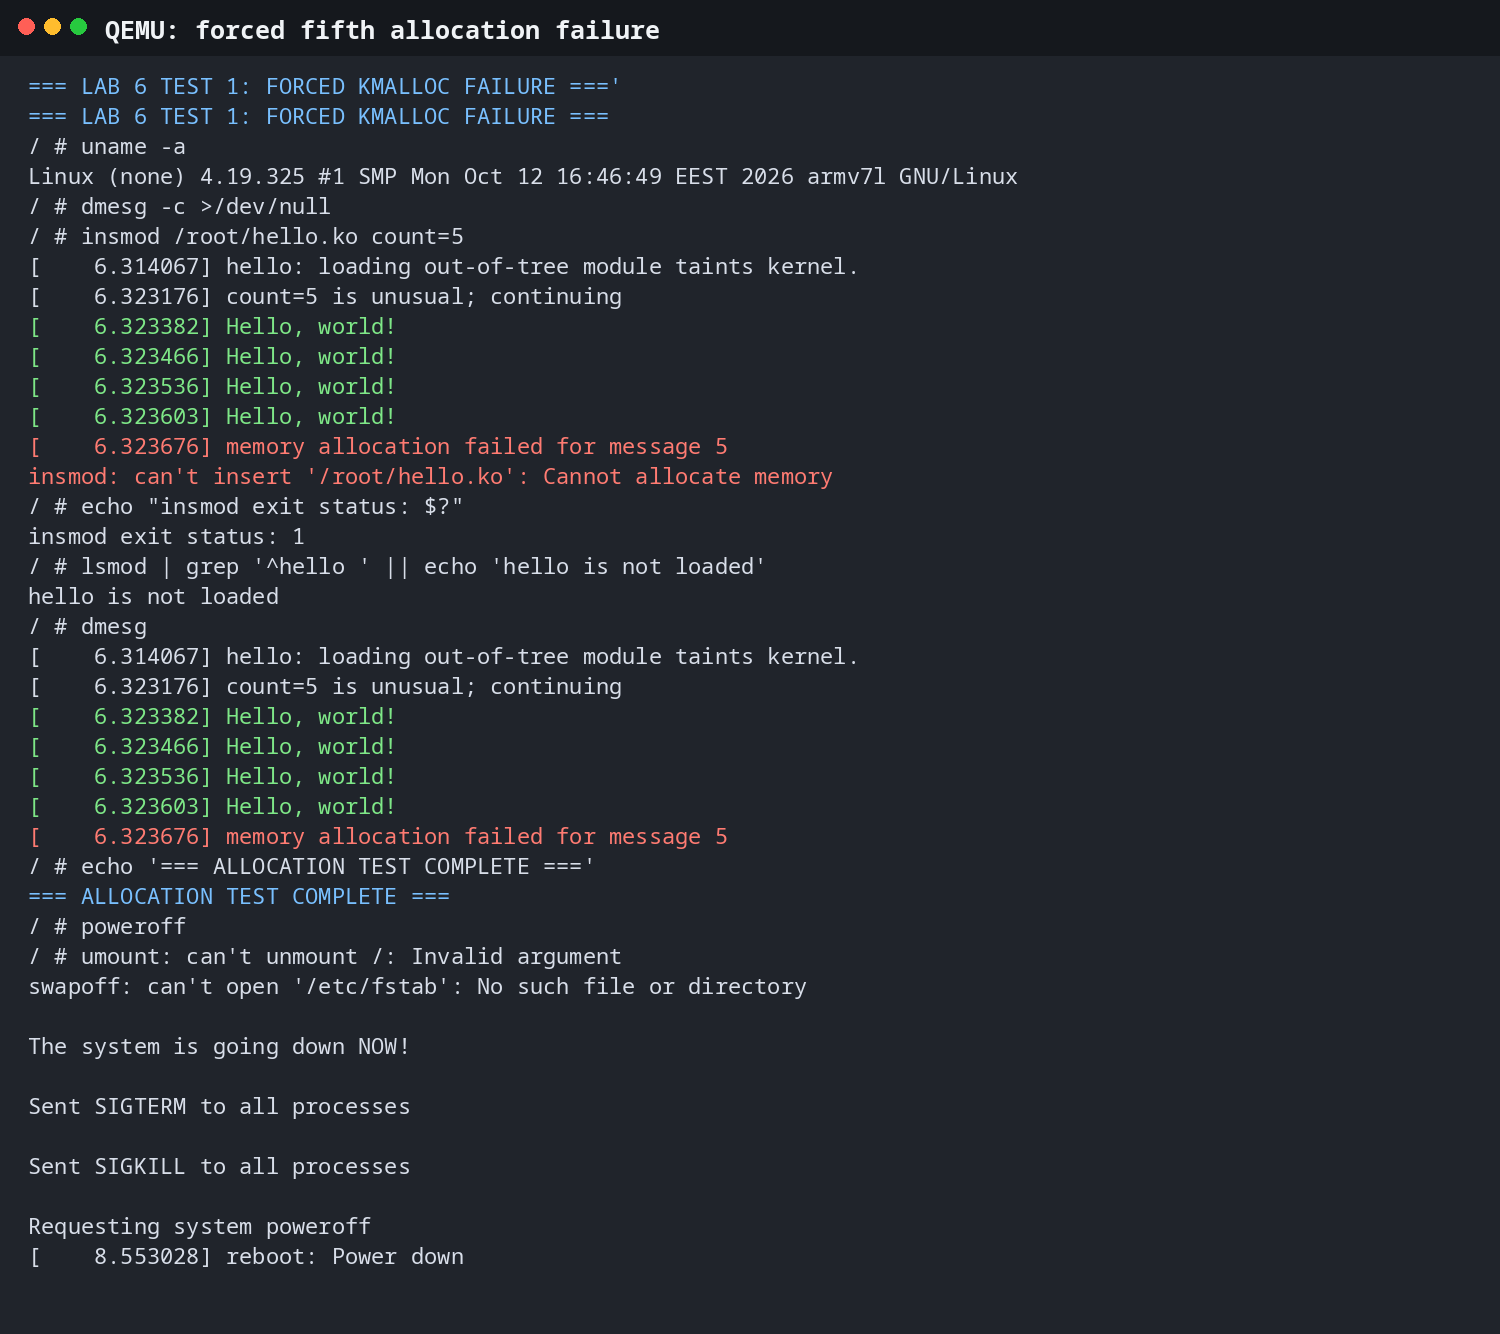
\includegraphics[width=0.76\textwidth]{media/forced-allocation-failure.png}
  \caption{Штучна відмова п'ятого виділення пам'яті}
\end{figure}

\subsection{BUG\_ON і стан модуля}

Для \texttt{count=11} ядро сформувало \texttt{Oops - BUG} і завершило
процес \texttt{insmod} сигналом сегментації зі статусом 139. У трасуванні
вказано \texttt{hello\_init+0x18}, адресу PC \texttt{0xbf005018} і рядок
\texttt{hello.c:43}. Команда \texttt{lsmod} показала модуль у стані
\texttt{Loading (O+)}, а спроба \texttt{rmmod hello} завершилася
повідомленням \texttt{Device or resource busy}.

\begin{figure}[H]
  \centering
  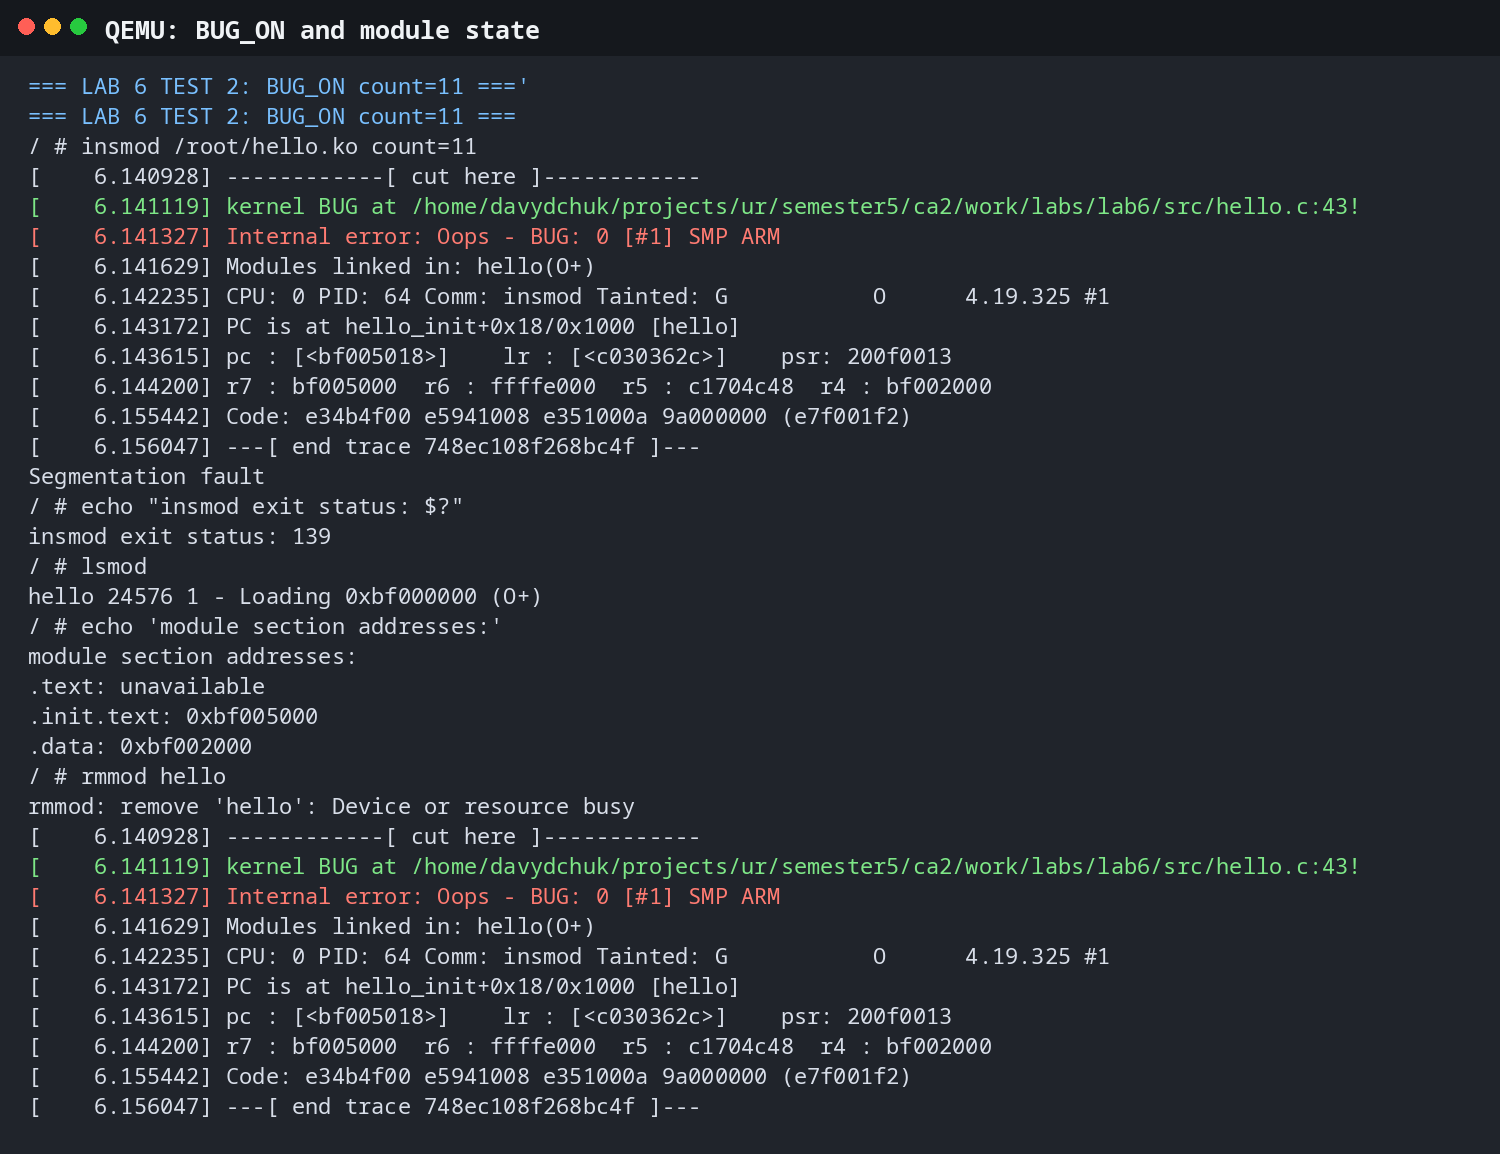
\includegraphics[width=0.88\textwidth]{media/bug-on-oops.png}
  \caption{Oops, адреси секцій і неможливість вивантаження модуля}
\end{figure}

\subsection{Пошук рядка аварії}

У sysfs прочитано базу секції \texttt{.init.text}:
\texttt{0xbf005000}. Віднімання її від PC дало зміщення \texttt{0x18}.
Команда \texttt{addr2line} визначила функцію \texttt{hello\_init} і рядок
43, де розміщено \texttt{BUG\_ON(count > 10)}.

Дизасемблювання підтвердило результат: після порівняння параметра з 10 і
умовного переходу за зміщенням \texttt{0x18} знаходиться аварійна ARM-
інструкція \texttt{0xe7f001f2}.

\begin{figure}[H]
  \centering
  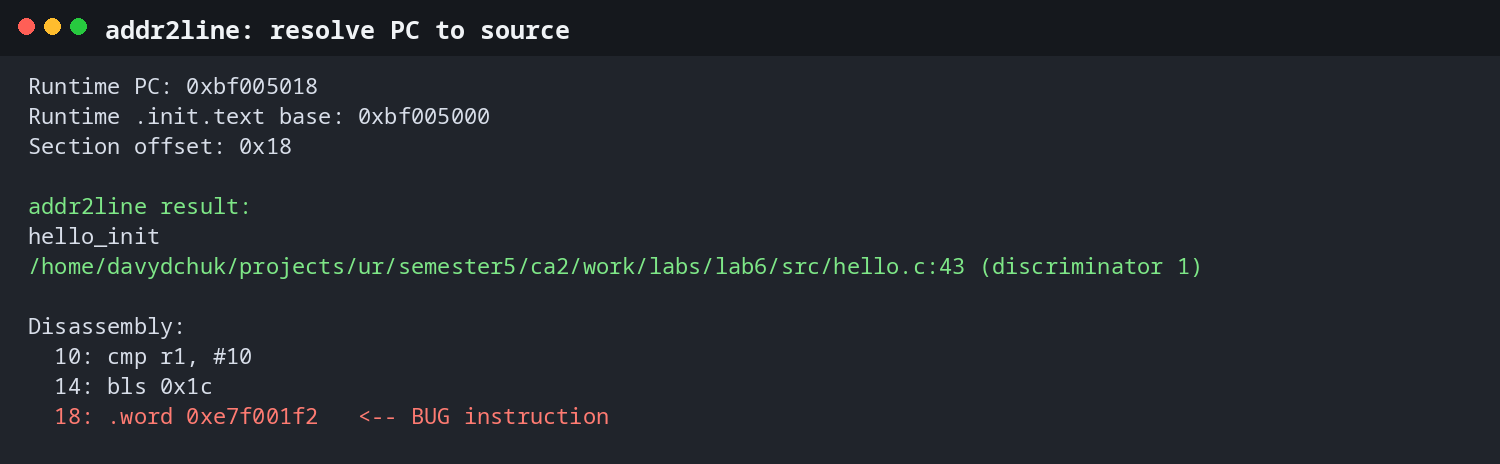
\includegraphics[width=\textwidth]{media/address-resolution.png}
  \caption{Обчислення зміщення та визначення рядка через addr2line}
\end{figure}

Повні журнали двох сесій QEMU, дизасемблювання та результат
\texttt{addr2line} збережено у каталозі \texttt{evidence} у форматах TXT
і HTML.

\section{Висновки}

У роботі реалізовано й досліджено два різні класи помилок модуля ядра.
Штучна відмова виділення пам'яті була коректно оброблена поверненням
\texttt{-ENOMEM}: модуль не завантажився, але стан ядра не було порушено.
Неприпустимий параметр активував \texttt{BUG\_ON()}, створив Oops і залишив
модуль зайнятим у проміжному стані.

За адресою PC та базою \texttt{.init.text} обчислено зміщення
\texttt{0x18}. Засоби \texttt{addr2line} й \texttt{objdump} однозначно
зіставили його з рядком 43 вихідного коду та аварійною інструкцією ARM.
Отже, практично відпрацьовано читання Oops, sysfs-секцій і пошук місця
аварії у зовнішньому модулі.

\section*{Використані матеріали}

\begin{enumerate}[leftmargin=*]
  \item Методичні вказівки до лабораторної роботи №6.
  \item Вихідний код Linux 4.19.325: \path{include/linux/bug.h}.
  \item Документація ядра: \path{Documentation/filesystems/sysfs.txt}.
  \item Linux Kernel Labs, Kernel modules: \url{https://linux-kernel-labs.github.io/refs/heads/master/labs/kernel_modules.html}.
\end{enumerate}

\newpage
\section*{Додаток А. Вихідний код hello.c}
\addcontentsline{toc}{section}{Додаток А. Вихідний код hello.c}

\VerbatimInput[fontsize=\tiny,breaklines=true,breakanywhere=true,frame=single,framesep=2mm]{../src/hello.c}

\newpage
\section*{Додаток Б. Kbuild і Makefile}
\addcontentsline{toc}{section}{Додаток Б. Kbuild і Makefile}

\subsection*{Kbuild}
\VerbatimInput[fontsize=\small,frame=single,framesep=2mm]{../src/Kbuild}

\subsection*{Makefile}
\VerbatimInput[fontsize=\small,breaklines=true,frame=single,framesep=2mm]{../src/Makefile}

\end{document}
